\begin{frame}
\tableofcontents

\printnoidxglossary[type=\acronymtype,title=List of Abbreviations]
\listoffigures

\mainmatter
\end{frame}

\begin{frame}{Introduction}
\protect\hypertarget{introduction}{}
\end{frame}

\begin{frame}[fragile]{Related work}
\protect\hypertarget{related-work}{}
This chapter explores prior work related to multi-party connectivity
over The Internet and their suitability for joint MPyC computations.
Section \ref{sec:internet} provides an overview of the protocols of the
modern Internet, the challenges for Peer-to-Peer communications and some
of the approaches to overcome them. Section \ref{sec:overlays} discusses
higher-level network overlays that use different combinations of the
lower-level protocols from the previous section.

\begin{block}{The Internet}
\protect\hypertarget{sec:internet}{}
The Internet is a global multi-tiered computer network of billions of
host devices that communicate using the protocols of the Internet
Protocol Suite (TCP/IP). \glspl{isp} are responsible for managing
different sections of the infrastructure that connects the \glspl{lan}
of various end-users including households and enterprises. The \gls{www}
or simply The Web is a collection of interconnected documents, e.g.~HTML
Web Pages, available on The Internet and is typically accessed via a
user-agent software such as a \textbf{\emph{Web Browser}}. The term
``The Web'' is sometimes used interchangeably with The Internet, but The
Internet supports other services as well, e.g.~file transfer (FTP),
email (IMAP), instant messaging, remote access (SSH) and others.
Conceptual frameworks like the OSI model are useful for understanding
the objectives and functions of communication protocols. Figure
\ref{osi-map-tcp} describes the responsibilities of the 7 layers of the
OSI model and how they relate to the TCP/IP model used by the Internet
Protocol Suite. The newer TCP/IP model only recognizes 4 layers as it
merges the OSI Session (L5) and Presentation (L6) layers into the
Application layer (L7), as well as the Physical layer (L1) into the Data
link layer (L2). While the TCP/IP model is a more accurate
representation of The Internet, the 7-layer numbers of the OSI model are
still widely used in the literature.

\begin{figure}
\centering
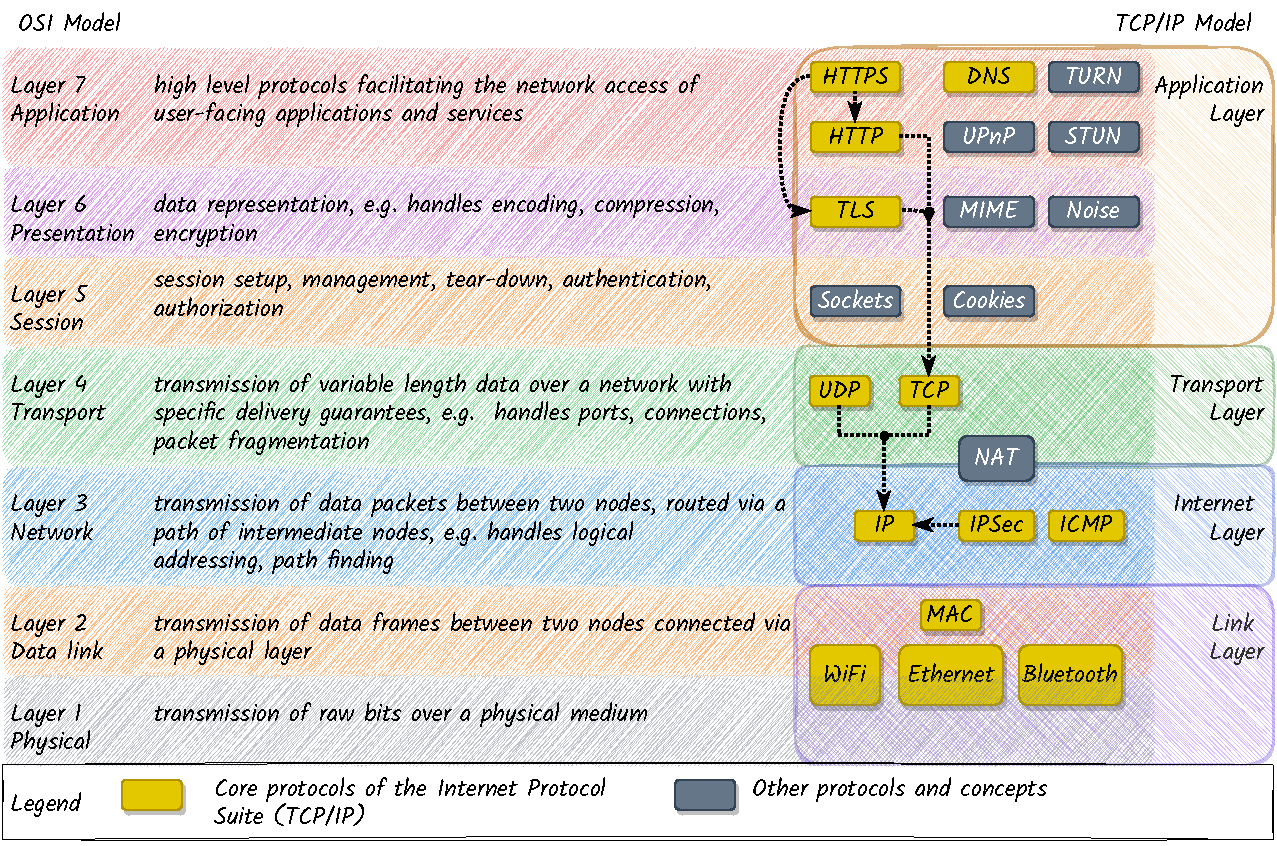
\includegraphics[width=1\textwidth,height=\textheight]{thesis/../figures/osi-map-tcp.drawio.pdf}
\caption{OSI model mapping of the Internet Protocol
Suite\label{osi-map-tcp}}
\end{figure}

\begin{block}{Communications}
\protect\hypertarget{communications}{}
The \textbf{\acrfull{ip}} is a Network (L3) protocol of the Internet
Protocol Suite that is responsible for delivering datagrams between
devices across the boundaries of their \glspl{lan} by possibly routing
traffic via multiple intermediate devices (routers). A datagram is a
connectionless packet that is delivered on a best-effort basis. IP
datagrams have a header that contains fields such as the \textbf{IP
addresses} of its source and destination, and a
\todo{show a diagram of the internet with multiple local networks}
payload that encapsulates the data from the protocols of the layers
above. Routers are devices that are part of multiple networks and relay
datagrams between them based on a routing table that maps IP address
ranges to networks. \textbf{\emph{\gls{cidr}}} is a common notation for
describing IP address ranges, e.g.~\texttt{192.168.0.1/16}, where the
number after the slash describes the bit-length of the fixed prefix for
a subnet.

\textbf{\acrfull{udp}} and \textbf{\acrfull{tcp}} are Transport layer
(L4) protocols that employ 16-bit port numbers to enable multiple
applications on the same host to establish their own communication
channels while sharing an IP address. UDP offers faster communication,
but only provides best-effort delivery, while TCP is a reliable
transport protocol with stronger delivery guarantees at the expense of
higher network latency. TCP maintains stateful connections that handle
error detection and correction, packet ordering, flow control,
acknowledgments and retransmissions in case packets are lost during
transmission.

\textbf{\emph{\gls{http}}} is an Application layer (L7) protocol used
for transmitting data on The Web between web servers and clients like
browsers, typically using a stateless request/response model. Similar to
other L7 protocols, it uses \textbf{\emph{\glspl{url}}} for identifying
resources using the format
\texttt{scheme://host:port/path?query=value\#fragment},
e.g.~http://www.example.com:80/path/to/file.html. It is built on top of
TCP and provides several features such as:

\begin{itemize}
\tightlist
\item
  Request Methods - used by the client to specify the action to perform
  on the resource behind the given URL, e.g.~GET, POST, PUT, DELETE,
  etc.
\item
  Headers - used to provide additional information about a request or
  response, e.g.~Content-Type, Authorization, Cache-Control
\item
  Status codes - used to indicate whether or not the result of a
  request, e.g.~if it was successful (200), or if the resource is
  missing (404)
\item
  Cookies - used to include stateful information about the user kept at
  the client-side
\item
  Caching - used to specify that the result of a request can be cached
  for a certain time to avoid repeating the request's action.
\end{itemize}

The \textbf{\emph{\gls{dns}}} operates at the Application Layer (L7) and
allows the conversion of human-readable domains to IP addresses,
e.g.~\texttt{google.com} to \texttt{142.250.179.142}.
\end{block}

\begin{block}{Host Addressing}
\protect\hypertarget{host-addressing}{}
The version of the Internet Protocol, that was originally deployed
globally (IPv4), uses 32-bit numbers as IP addresses, allowing for
around 4 billion unique addresses. Due to the popularity of The
Internet, there are many more devices than available IPv4 addresses,
which has caused challenges. IPv6 is a newer version of the protocol
that uses a larger 128-bit address space which is sufficient for
assigning 100 addresses for each atom on Earth. Its adoption has been
slow, as according to Google as of 2023 only around 37\% of the requests
to their services use IPv6. Additionally, despite that IPv6 allows for
all devices to be addressable on the Internet, for security reasons,
most of them would use firewalls to block incoming remote traffic that
is not associated with outgoing connections.

A widespread solution to the addressing problem is \textbf{\gls{nat}}.
It allows many devices without globally unique IP addresses to initiate
connections to publicly addressable devices on the Internet via a
limited number of gateways that must have globally unique IP addresses.
A NAT gateway replaces the local source IP address of each outgoing IP
datagram with its own public IP address before passing it on to the next
link on the way to the destination while maintaining a mapping between
the source and destination IPs in a translation table. The destination
host can then address its responses back to the NAT gateway's public IP
address, which in turn replaces its own IP from the incoming datagrams
with the IP of the local device and forwards them to it. If the IP
datagrams encapsulate TCP/UDP packets, the gateway additionally rewrites
the source and destination ports, which means that NAT techniques can be
placed somewhere between Layers 3 and 4 of the OSI model.

The effect of NAT on connectivity is similar to an IPv6 firewall as they
both allow devices on a local network to initiate bidirectional
communication to remote devices with public IP addresses, but
connections cannot be natively initiated by the remote devices. As
Figure \ref{nat-intro} shows, it follows that when two devices are
behind separate NATs, neither can contact the other first.
\textbf{Client/Server} communication is less affected by this limitation
because Servers are usually deployed to a public IP address that can be
contacted by Clients with local IP addresses. \textbf{Peer-to-Peer}
communication, however, is more challenging because the peers are often
devices in separate residential networks behind different NATs. Several
\textbf{NAT traversal} techniques try to solve this with different
performance tradeoffs and success that varies depending on the NAT
\autocite{natBehaviorRFC} and its behavior when mapping ports and IP
addresses.
\todo{describe some of the nat behaviors, e.g. if the source IP address/port vary per destination are changed depending on the destination/port mapping algorithms, if it maps ports, IPs, whether the mapped IPs are different per destination and others.}

\begin{figure}
\centering
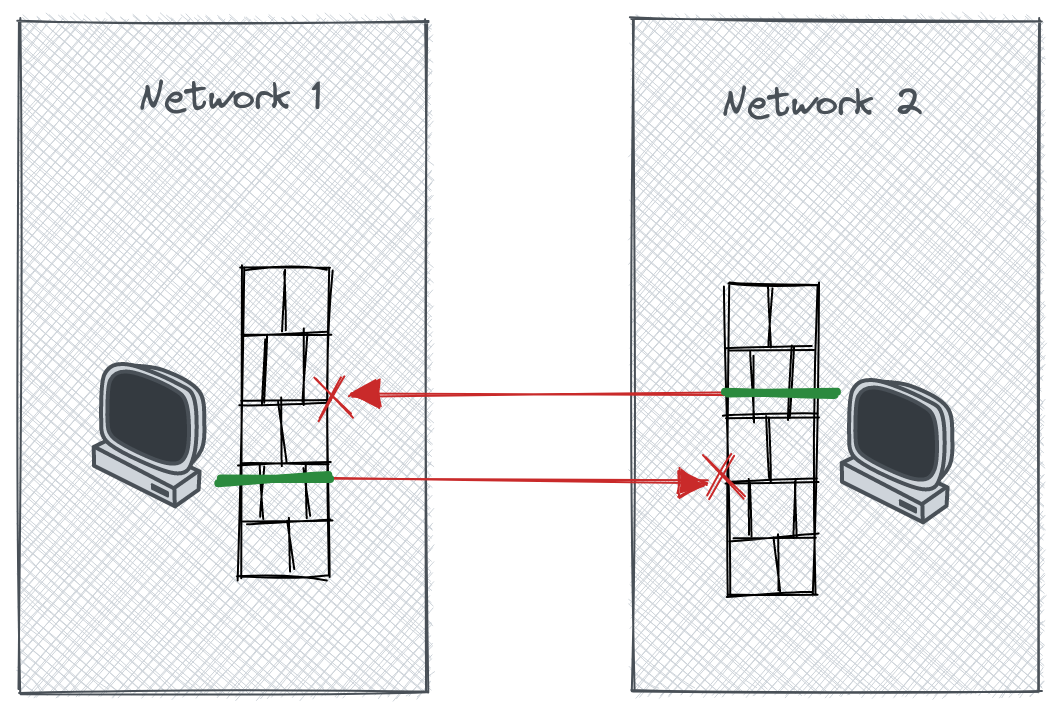
\includegraphics[width=\textwidth,height=0.25\textheight]{thesis/../figures/nat-intro.png}
\caption{Two parties behind separate NATs\label{nat-intro}}
\end{figure}

One approach based on the Client/Server model is to use a publicly
addressable \textbf{relay} server that is contacted by the NATed devices
and then forwards the Peer-to-Peer traffic to the intended recipient.
Compared to direct communication, relaying results in a higher network
latency due to the longer path that each packet must travel. Maintaining
a relay server requires some technical expertise and may be costly
depending on the expected throughput. Despite the drawbacks, relaying
works under most networking scenarios and is therefore often used as a
fallback in case all other approaches fail to find a direct path.
Protocols such as \textbf{\acrfull{turn}} \autocite{turnRFC} and
\textbf{\acrfull{derp}} \autocite{derpDocs} can be used to securely
implement relaying.

The NAT gateway in many residential networks is a Router device under
the customer's control that has a statically or dynamically assigned
public IP address. Most routers can be manually configured through their
admin page to forward all traffic that arrives at a given port to a
specific device on the local network. Remote applications can then
initiate a connection to the local device if they know the IP address of
the router and the forwarded port. The manual configuration, however,
can be inconvenient and many users may be unaware of that setting
because it is not necessary for the more straightforward Client/Server
communications. Some routers also support programmatic configuration of
port forwarding via a Layer 7 protocol like \textbf{\gls{upnp}} or its
successors \textbf{\gls{nat-pmp}} and \textbf{\gls{pcp}}. However, these
protocols are not always supported and are often disabled by the local
network administrators due to security concerns related to bugs in their
implementation, vulnerable IOT devices on the local network or malicious
programs being able to expose local devices to the internet.

An efficient NAT traversal approach that works with some types of NATs
is to use \textbf{\gls{stun}} \autocite{stunRFC} in combination with UDP
hole punching (Figure \ref{nat-traversal}). STUN is a protocol operating
at Layer 7 that allows a client application to detect the presence of
NAT gateways on the network path to a public STUN server, and identify
their types and the public IP address that they map to externally. An
application sends UDP datagrams to the STUN server and it responds with
the source IP address and port specified inside them. The application
can compare its own endpoint with the source endpoint observed by the
STUN server and if the values differ, it can be inferred that they were
rewritten by a NAT. Additional STUN servers are contacted to determine
if the NAT maps IPs and ports in a predictable fashion. UDP hole
punching is a related technique that, depending on the NAT types, can
allow direct communication between two applications behind separate
NATs. The applications must discover each other's externally mapped
endpoints, perhaps via the STUN server. If the NATs use the same
external port regardless of the remote destination, the two applications
can simultaneously send UDP packets to each other's external endpoints.
Their respective NATs will see the outgoing connection to the other peer
- the ``punched hole'' - when the incoming traffic arrives from it and
forward it correctly. NATs that map different ports per remote
destination sometimes allocate port numbers predictably, which can be
used by the peers to try to guess the port that will be opened by the
opposing side's NAT.

\begin{figure}
\centering
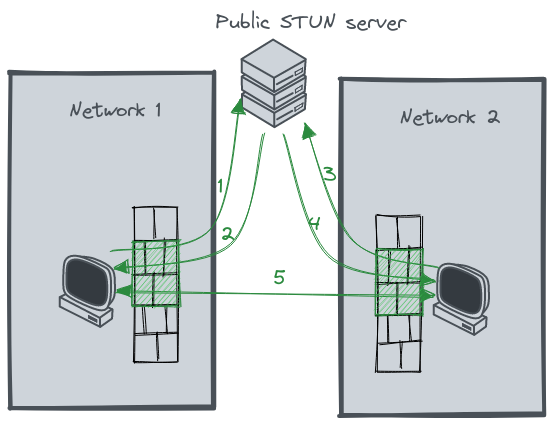
\includegraphics[width=\textwidth,height=0.25\textheight]{thesis/../figures/nat-traversal.png}
\caption{NAT traversal via STUN\label{nat-traversal}}
\end{figure}

In mobile networks like 4G and 5G, the \gls{isp} often utilizes a
\textbf{\gls{cgnat}} as part of their infrastructure, while all devices
under the user's control, including the router, only have local IP
addresses. STUN techniques would fail to discover a direct path between
two parties behind separate CGNATs or other unpredictable NAT
algorithms. The only remaining possibility is to relay the traffic via a
publicly reachable third-party host.
\todo{only ~65000 ports per IP address means that CGNATs that provide more than 65000 connections from client devices require more than one public IP address}

\todo{hairpinning - Hairpinning, also known as NAT loopback or NAT reflection, is a technique used by NAT devices to allow hosts on a private network to access a public server using its public IP address. Without hairpinning, the NAT device would not recognize the connection as a loopback connection and would route it to the public network, causing the connection to fail. With hairpinning, the NAT device recognizes that the connection is a loopback connection and redirects the traffic back to the same NAT device, which then forwards the traffic to the correct host on the private network. This can be useful in scenarios where a private network is hosting a public-facing server that is also accessed by internal users on the same network using its public IP address.}
\end{block}

\begin{block}{Security}
\protect\hypertarget{security}{}
\textbf{\acrfull{tls}} is a protocol that adds encryption on top of a
reliable transport protocol such as TCP. It is a successor to \gls{ssl}.
TLS does not strictly fit in any single OSI layer, but is usually placed
somewhere between the Transport Layer (L4) and the Presentation Layer
(L6). It is rather complex because it needs to support many possible use
cases across the internet. \todo{tls certificates} The \textbf{Noise
Protocol Framework} \autocite{noiseDocs} is a more
\todo{noise is transport agnostic}
\todo{noise has limited cipher suites} recent effort that applies the
ideas of TLS in a simplified way by serving as a blueprint for designing
use-case specific protocols for establishing secure communication
channels based on \gls{ecdh} handshake patterns. It powers the
end-to-end encryption in messaging applications such as WhatsApp and
Signal, and \gls{vpn} software such as WireGuard and Nebula.

\textbf{\emph{HTTPS}} uses TLS to encrypt the HTTP traffic between a
client and a server.

\todo{talk about https}

\textbf{\acrfull{ipsec}} is a protocol suite for encrypting the IP
datagrams between two hosts. It was originally developed as part of IPv6
but can also be used with IPv4. IPSec is similar in purpose to TLS but
operates at the Network Layer (L3).

\todo{tls requires the clients to be configured with a certificate for the server, IPSec needs to server to also be configured with a certificate for the client.}

\todo{tls works in browsers, IPSec works at the OS level}

\todo{The Internet Protocol Security (IPSec) protocol suite is designed specifically to provide secure communication between two hosts at the network layer (L3) of the OSI model. IPSec can be used to secure traffic between two hosts, between a host and a network, or between two networks. It provides a range of services, including data confidentiality, data integrity, and authentication, and is often used in Virtual Private Network (VPN) connections to create secure tunnels between remote networks. IPSec operates in either Transport or Tunnel mode, and can use either the Authentication Header (AH) or Encapsulating Security Payload (ESP) protocols to provide its security services.}

\begin{itemize}
\tightlist
\item
  \textbf{\acrfull{ipsec}}

  \begin{itemize}
  \tightlist
  \item
    Layer 3 protocol suite part of the Internet Protocol Suite
  \item
    used inside VPN software
  \item
    has implementations in both user and kernel space as well as
    hardware implementations
  \item
    rewrites and encrypts the IP headers and payloads
  \item
    virtual routing table
  \item
    Initially was built into IPv6, separate from IPv4
  \end{itemize}
\end{itemize}
\end{block}
\end{block}

\begin{block}{Network overlays}
\protect\hypertarget{sec:overlays}{}
Most Network Overlay solutions use a combination of the NAT traversal
techniques mentioned previously. They can be placed in Layers 2, 3 or 7.
Layer 2 overlays act as a virtual network switch, while Layer 3 overlays
act as a virtual network router. Layer 7 overlays are implemented in
user-space as libraries or applications that run on top of the network
stack of the host operating system. Layer 2 and 3 overlays can either be
implemented as kernel modules or as user-space applications that use a
\textbf{TUN/TAP} driver to interface with the kernel.

Figure \ref{osi-map-overlays} shows an approximate OSI model mapping of
several protocols and network overlay solutions from the point of view
of the systems that use them and the arrows show dependency relations
between them.

\begin{figure}
\centering
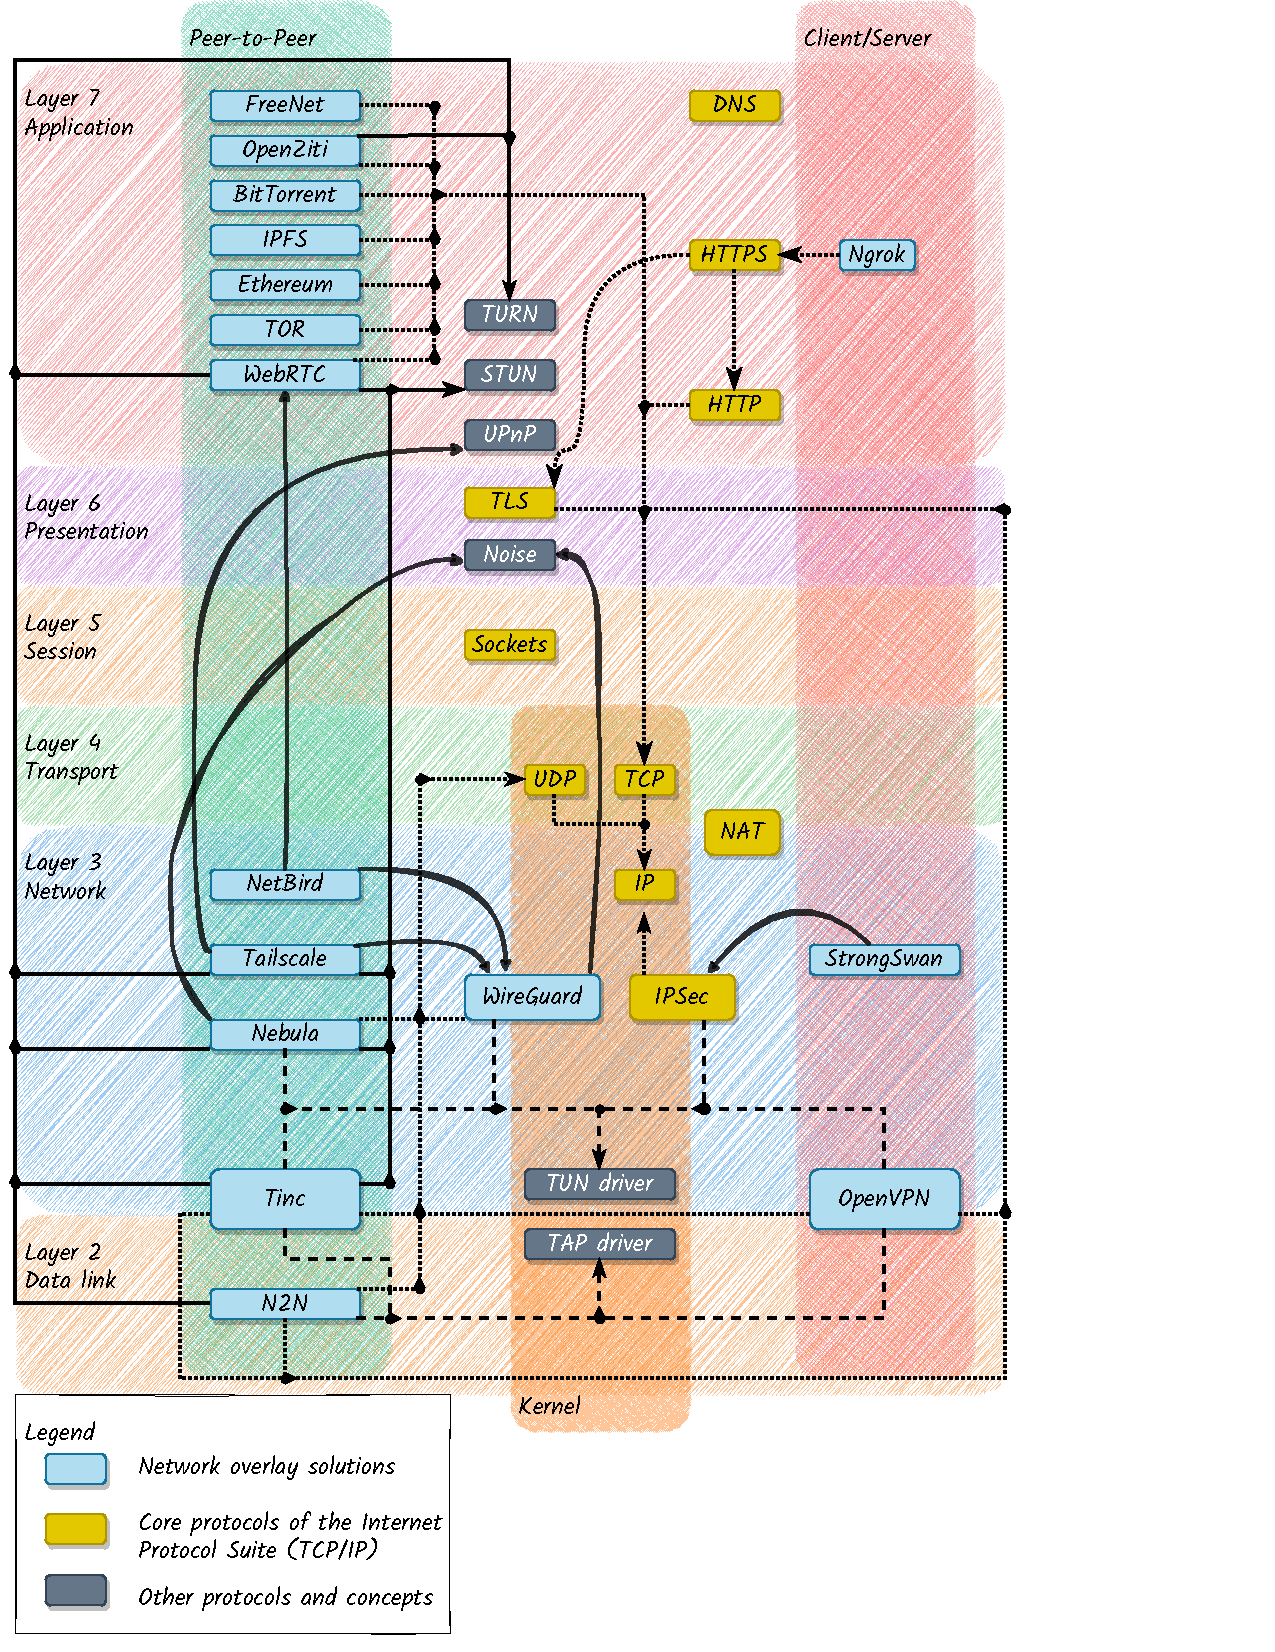
\includegraphics[width=\textwidth,height=0.9\textheight]{thesis/../figures/osi-map-overlays.drawio.pdf}
\caption{OSI model mapping of various protocols
\label{osi-map-overlays}}
\end{figure}

\begin{block}{TUN/TAP driver}
\protect\hypertarget{tuntap-driver}{}
\begin{itemize}
\tightlist
\item
  Layer 2 vs Layer 3 Networks

  \begin{itemize}
  \tightlist
  \item
    Layer 2 overlays bridge networks

    \begin{itemize}
    \tightlist
    \item
      virtual network switch
    \item
      remote machines are on the same virtual LAN and can share the same
      IP address range
    \item
      allows broadcast/multicast
    \item
      TAP driver
    \end{itemize}
  \item
    Layer 3 overlays route traffic between separate local networks

    \begin{itemize}
    \tightlist
    \item
      virtual network router
    \item
      remote machines are on separate LANs
    \item
      simpler to configure
    \item
      TUN driver
    \end{itemize}
  \end{itemize}
\end{itemize}
\end{block}

\begin{block}{Traditional VPNs}
\protect\hypertarget{traditional-vpns}{}
\todo{tls vs ipsec vpns. TLS vpns offer a virtual network interface at layer 3, but run over L7 TLS }

\glspl{vpn} are implemented as Layer 2 or 3 network overlays. They are
commonly used for securely connecting machines from different
\glspl{lan}. They provide software emulation of a network interface
controller via a TUN/TAP driver on the operating system level and allow
other software to transparently use the functionality of the \gls{ip}
suite without requiring extra changes. Traditional \glspl{vpn} such as
IPSec \autocite{ipSecDocs} and OpenVPN \autocite{openVPNDocs} use a
centralized service that all (encrypted) client communications must pass
through. This introduces a single point of failure and a potential
bottleneck that might negatively impact the performance of the
multi-party computations due to their \gls{p2p} nature.
\end{block}

\begin{block}{WireGuard}
\protect\hypertarget{wireguard}{}
WireGuard \autocite{donenfeldWireGuardNextGeneration2017} is a more
recent protocol with a design informed by lessons learned from IPSec and
OpenVPN and a key management approach inspired by SSH. It is a
lower-level protocol that focuses on configuration simplicity while
network topology, peer discovery and key distribution are left as a
responsibility of higher-level systems that use it as a building block.
Wireguard is implemented as a Layer 3 overlay over UDP tunnels.
WireGuard has both user-space implementations that use a TUN driver and
also has direct support built into the Linux Kernel since version 5.6
(May 2020). The kernel implementation allows for better performance
because it does not need to copy packets between the kernel and
user-space memory.

The snippets below show a minimal set of configuration options that need
to be provided for two peers to be able to form secure tunnels with each
other.

\begin{Shaded}
\begin{Highlighting}[]
\CommentTok{\# peer1.conf}
\KeywordTok{[Interface]}
\DataTypeTok{Address }\OtherTok{=}\StringTok{ 101.0.0.1/32}
\DataTypeTok{ListenPort }\OtherTok{=}\StringTok{ }\DecValTok{53063}
\DataTypeTok{PrivateKey }\OtherTok{=}\StringTok{ ePTiXXhHjvAHdWUr8Bimk30n0gh3m241RAzsN0JZDW0=}

\KeywordTok{[Peer]}
\DataTypeTok{PublicKey }\OtherTok{=}\StringTok{ BSn0ejd1Y3bKuD+Xpg0ZZeOf+Ies/oql0NZxw+SOmkc=}
\DataTypeTok{AllowedIPs }\OtherTok{=}\StringTok{ 101.0.0.2/32}
\DataTypeTok{Endpoint }\OtherTok{=}\StringTok{ peer1.example.com:38133}
\end{Highlighting}
\end{Shaded}

\begin{Shaded}
\begin{Highlighting}[]
\CommentTok{\# peer2.conf}
\KeywordTok{[Interface]}
\DataTypeTok{Address }\OtherTok{=}\StringTok{ 101.0.0.2/32}
\DataTypeTok{ListenPort }\OtherTok{=}\StringTok{ }\DecValTok{38133}
\DataTypeTok{PrivateKey }\OtherTok{=}\StringTok{ sN/d6XUPEVPGSziVgCCOnOivDK+qAoYC3nxnssQ5Rls=}

\KeywordTok{[Peer]}
\DataTypeTok{PublicKey }\OtherTok{=}\StringTok{ e/TxvPmrgcc1G4cSH2bHv5J0PRHXKjYxTFoU8r+G93E=}
\DataTypeTok{AllowedIPs }\OtherTok{=}\StringTok{ 101.0.0.1/32}
\end{Highlighting}
\end{Shaded}

Each peer has a public/private key pair that is used for authentication
and encryption based on the Noise Protocol Framework
\autocite{noiseDocs}. The \texttt{Address} field specifies the virtual
IP address that the local network interface will use, while the
\texttt{AllowedIPs} field specifies what virtual IP addresses are
associated with a peer's public key. A peer's \texttt{Endpoint} field
specifies the URL at which it can be reached. Only one of the peers must
be configured with a reachable endpoint for the other one. In the above
example once \texttt{peer1} initiates communication with \texttt{peer2},
\texttt{peer2} will learn the current endpoint of \texttt{peer1} and
will be able to communicate back with it.
\end{block}

\begin{block}{Mesh VPNs}
\protect\hypertarget{mesh-vpns}{}
\begin{itemize}
\tightlist
\item
  Tinc
\item
  N2N
\item
  Tailscale
\item
  Nebula
\item
  ZeroTier
\end{itemize}

Mesh \glspl{vpn} such as Tinc \autocite{tincDocs}, Tailscale
\autocite{tailscaleDocs} and Nebula \autocite{nebulaDocs} utilize NAT
Traversal techniques to create direct \gls{p2p} links between the
clients for the data traffic. Authentication, authorization and traffic
encryption are performed using certificates based on public key
cryptography.

All three are open-source, except Tailscale's coordination service which
handles peer discovery and identity management. Headscale
\autocite{fontJuanfontHeadscale2022} is a community-driven open-source
alternative for that component. Tinc is the oldest of the three but has
a relatively small community. It is mainly developed by a single author
and appears to be more academic than industry motivated. Nebula and
Tailscale are both business driven. Tailscale was started by some
high-profile ex-googlers and is the most end-user-focused of the three,
providing a service that allows people to sign up using identity
providers such as Google, Microsoft, GitHub and others. They also
provide an Admin console that allows a user to easily add their personal
devices to a network or share them with others. It also has support for
automation tools like Terraform for creating authorization keys and
managing an \gls{acl} based firewall. Nebula was originally developed at
the instant messaging company Slack to create overlay networks for their
cross-region cloud infrastructure, but the authors later started a new
company and are currently developing a user-centric platform similar to
Tailscale's. Nebula is more customizable than Tailscale and since it is
completely open-source it can be adapted to different use cases, but it
is also more involved to set up. A certificate authority needs to be
configured for issuing the identities of the participating hosts.
Furthermore, publicly accessible coordination servers need to be
deployed to facilitate the host discovery. Tailscale employs a
distributed relay network of \gls{derp} servers, while Nebula can be
configured to route via one of the other peers in the VPN.
\end{block}

\begin{block}{Layer 7 overlays}
\protect\hypertarget{layer-7-overlays}{}
\begin{block}{WebRTC is}
\protect\hypertarget{webrtc-is}{}
\begin{itemize}
\tightlist
\item
  WebRTC

  \begin{itemize}
  \tightlist
  \item
    Uses STUN/TURN
  \item
    d
  \end{itemize}
\item
  OpenZiti

  \begin{itemize}
  \tightlist
  \item
    uses relays
  \end{itemize}
\item
  ngrok
\item
  TOR
\item
  BitTorrent
\item
  IPFS
\item
  Ethereum
\item
  Teleport
\item
  Freenet
\end{itemize}
\end{block}
\end{block}
\end{block}
\end{frame}

\begin{frame}{Testing methodology}
\protect\hypertarget{testing-methodology}{}
In the following chapters, we will design and implement several
solutions for ad hoc MPC sessions based on a subset of the previously
discussed related works:

\begin{itemize}
\tightlist
\item
  Internet protocol
\item
  Wireguard
\item
  Tailscale
\item
  Headscale
\item
  ? Headscale with DID identity?
\item
  ? WebRTC?
\item
  A custom solution that automates the WireGuard configuration by
  visiting a web page
\end{itemize}

Additionally, we will analyze and compare them in terms of performance,
security and usability

\begin{block}{Measuring performance}
\protect\hypertarget{measuring-performance}{}
During the preparation phase of the project, we developed the \gls{e3}
framework which simplifies and automates the process of deploying
machines in different geographical regions, connecting them via an
overlay network and executing multiparty computations between them,
where each machine represents a different party.

To summarize, \gls{e3} is a set of scripts that use several automation
tools:

\begin{itemize}
\tightlist
\item
  Terraform - declarative provisioning
\item
  NixOS - declarative Linux distribution
\item
  Colmena - declarative deployment for NixOS
\item
  PSSH - parallel execution of remote scripts over ssh
\item
  DigitalOcean - a cloud provider
\end{itemize}

It allows us to quickly provision cloud virtual machines in multiple
regions and reproducibly deploy all necessary software for running a
multiparty computation over a chosen network overlay solution. The
source code of \gls{e3} can be found on
\href{https://github.com/e-nikolov/mpyc}{GitHub}

Each solution will be deployed using the \gls{e3} framework and the
performance will be quantitatively measured in terms of the time it
takes to execute several MPyC demos. The selected demos have different
complexities in terms of communication rounds and message sizes which
will allow us to observe their impact on the overall performance.

\begin{enumerate}
\tightlist
\item
  Secret Santa - high round complexity with small messages
\item
  Convolutional Neural Network (CNN) MNIST classifier - low round
  complexity with large messages
\end{enumerate}

The demos will be configured at three different input size levels

\begin{itemize}
\tightlist
\item
  Low,
\item
  Medium
\item
  High
\end{itemize}

Furthermore, the demos will be executed in several networking scenarios:

\begin{enumerate}
\tightlist
\item
  1-10 parties in the same geographic region
\item
  1-10 parties evenly distributed across two nearby regions
\item
  1-10 parties evenly distributed across two distant regions
\item
  1-10 parties distributed across multiple distant regions
\end{enumerate}
\end{block}

\begin{block}{Security}
\protect\hypertarget{security}{}
We will analyze aspects such as

\begin{itemize}
\tightlist
\item
  key distribution
\item
  trust model - are there any trusted third parties and what would be
  the consequences if they are corrupted or breached
\item
  traffic encryption
\item
  identity strength
\end{itemize}
\end{block}

\begin{block}{Usability}
\protect\hypertarget{usability}{}
For each solution, we will describe the steps that the parties need to
perform to execute a joint multiparty computation. Those steps will be
analyzed in terms of:

\begin{itemize}
\tightlist
\item
  Complexity - how much technical expertise is expected from the parties
  to be able to execute the steps
\item
  Initial effort - how much effort is each party expected to put in
  preparing for their first joint computation
\item
  Repeated effort - after the initial setup, how much effort is required
  to perform another computation

  \begin{itemize}
  \tightlist
  \item
    with the same set of parties
  \item
    with another set of parties
  \end{itemize}
\item
  Finalization effort - how much effort is required to finalize the MPC
  session once it is complete and clean up any left-over artifacts or
  resources so that the machine of each party is in its original state
\end{itemize}
\end{block}
\end{frame}

\begin{frame}{Internet Protocol based solution}
\protect\hypertarget{internet-protocol-based-solution}{}
This solution focuses on directly using the internet protocol without
involving an overlay network. Our goal is to analyze the implications of
using only the functionalities that MPyC directly supports to serve as
the reference for our later experiments.

\begin{block}{Implementation details}
\protect\hypertarget{implementation-details}{}
We will manually set up the multiparty computations via the public IP
addresses of the machines and DNS.
\end{block}

\begin{block}{Performance analysis}
\protect\hypertarget{performance-analysis}{}
\end{block}

\begin{block}{Security analysis}
\protect\hypertarget{security-analysis}{}
\end{block}

\begin{block}{Usability analysis}
\protect\hypertarget{usability-analysis}{}
\end{block}
\end{frame}

\begin{frame}{WireGuard based solution}
\protect\hypertarget{wireguard-based-solution}{}
This solution creates an overlay network by manually configuring
WireGuard on each machine.

\begin{block}{Implementation details}
\protect\hypertarget{implementation-details}{}
\end{block}

\begin{block}{Performance analysis}
\protect\hypertarget{performance-analysis}{}
\end{block}

\begin{block}{Security analysis}
\protect\hypertarget{security-analysis}{}
\end{block}

\begin{block}{Usability analysis}
\protect\hypertarget{usability-analysis}{}
\end{block}
\end{frame}

\begin{frame}{Tailscale based solution}
\protect\hypertarget{tailscale-based-solution}{}
Tailscale is a VPN solution that configures a mesh of direct Wireguard
tunnels between the peers.

\begin{block}{Implementation details}
\protect\hypertarget{implementation-details}{}
\end{block}

\begin{block}{Performance analysis}
\protect\hypertarget{performance-analysis}{}
\end{block}

\begin{block}{Security analysis}
\protect\hypertarget{security-analysis}{}
\begin{block}{Trust model}
\protect\hypertarget{trust-model}{}
There is a centralized service that deals with the key distribution,
which needs to be trusted to provide the correct public keys for the
correct parties
\end{block}

\begin{block}{Identity}
\protect\hypertarget{identity}{}
Identity is based on third party identity providers such as Microsoft
and GitHub

\begin{itemize}
\item
  Magic DNS
\item ~
  \hypertarget{usability-analysis}{%
  \section{Usability analysis}\label{usability-analysis}}
\end{itemize}

With tailscale each party needs to

\begin{itemize}
\tightlist
\item
  register a Tailscale account
\item
  Download and install tailscale on the machine they want to run a
  multiparty computation
\item
  Run tailscale on their machine and logs into their account in order to
  link it to their own Tailnet
\item
  Share their Tailscale machine with the Tailnets of each of the other
  parties
\item
  Download the demo they want to run
\item
  Form the flags for running the chosen demo

  \begin{itemize}
  \tightlist
  \item
    add -P \$HOST:\$PORT for each party using their Tailscale
    hostname/virtual IP
  \end{itemize}
\item
  Run the demo
\end{itemize}
\end{block}
\end{block}
\end{frame}

\begin{frame}{Headscale based solution}
\protect\hypertarget{headscale-based-solution}{}
This solution is similar to the Tailscale one, but it uses Headscale - a
self-hosted open-source alternative to the closed-source Tailscale
coordination service.

\begin{block}{Implementation details}
\protect\hypertarget{implementation-details}{}
\end{block}

\begin{block}{Performance analysis}
\protect\hypertarget{performance-analysis}{}
\end{block}

\begin{block}{Security analysis}
\protect\hypertarget{security-analysis}{}
\begin{block}{Trust model}
\protect\hypertarget{trust-model}{}
There still is a centralized service like in the Tailscale solution, but
here it is self-deployed.
\end{block}

\begin{block}{Identity}
\protect\hypertarget{identity}{}
\end{block}
\end{block}

\begin{block}{Usability analysis}
\protect\hypertarget{usability-analysis}{}
\end{block}
\end{frame}
